% Nome do capítulo
\chapter{Trabalhos Relacionados}
\label{cap:3}
\vspace{-1.9cm}

Neste capítulo serão apresentados os trabalhos na literatura que possuem relação com o trabalho proposto.

\section{DenseNet}
\label{secao:3:1}

Como mencionado anteriormente, desde 2012 as tarefas de classificação de imagens são resolvidas majoritariamente por arquiteturas de \textit{Deep Learning}. Em \citeyear{he-2016}, \citeauthor{he-2016} propuseram a \ac{ResNet} que introduziam o conceito de \textit{skip connection}. Uma \textit{skip connection} é quando a camada $C_n$ além de se conectar com a camada $C_{n+1}$ ela se conecta com outra mais a frente - no caso da \textit{\ac{ResNet}}, a camada $C_{n+3}$. Sendo assim, a camada $C_{n+3}$ recebe em suas entradas uma junção das saídas de $C_{n}$ e $C_{n+2}$. Essa combinação de entradas na \ac{ResNet} foi feita como uma soma de matrizes. A Figura \ref{fig:blocoresidual} mostra um exemplo de \textit{skip connection} na \textit{\ac{ResNet}}.

\begin{figure}[H]
	% Alterar espaçamentos antes e depois do caption
	\setlength{\abovecaptionskip}{0pt}
	\setlength{\belowcaptionskip}{0pt}
	% Caption
	\caption[Exemplo de bloco residual]{Exemplo de bloco residual}
	\centering
	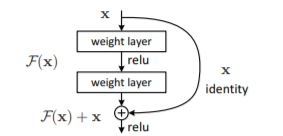
\includegraphics[width=.5\textwidth]{imagem/0x_resnet_arch.jpg}
	% Caption centralizada
	\captionsetup{justification=centering}
	\captionfont{\small{\textbf{\\Fonte: \citeonline{he-2016}.}}}	
	\label{fig:blocoresidual}
\end{figure}

Seguindo a mesma ideia de \textit{skip connection} proposta por \citeonline{he-2016}, \citeonline{liu-2017} propuseram a \ac{DenseNet}. Nessa nova arquitetura houveram duas mudanças com relação à \ac{ResNet}. A primeira mudança é que as saídas das camadas não seriam mais somadas, mas sim concatenadas, ou empilhadas. A segunda é que em um bloco residual as camadas se conectam com todas as suas sucessoras. 

A Figura \ref{fig:blocodenso} mostra como se conectam as camadas na \ac{DenseNet}. Supondo que temos um bloco denso $B$ com um conjunto de 5 camadas $C = \{c_1, c_2, c_3, c_4, c_5\}$. Como explicado no parágrafo anterior, a saída das camadas serão utilizadas em todas as camadas subsequentes no mesmo bloco. Sendo assim, a entrada de $c_3$ será composta pelas saídas de $c_1$ e $c_2$ concatenadas, e assim sucessivamente. Além disso, como as saídas são concatenadas e não somadas, a tendência é que as entradas cresçam a medida que a rede se aprofunda. O conceito de bloco denso permite propagar múltiplos níveis de abstração ao longo de toda a rede, melhorando assim os resultados obtidos \cite{liu-2017}.

\begin{figure}[H]
	% Alterar espaçamentos antes e depois do caption
	\setlength{\abovecaptionskip}{0pt}
	\setlength{\belowcaptionskip}{0pt}
	% Caption
	\caption[Exemplo de bloco denso]{Exemplo de bloco denso}
	\centering
	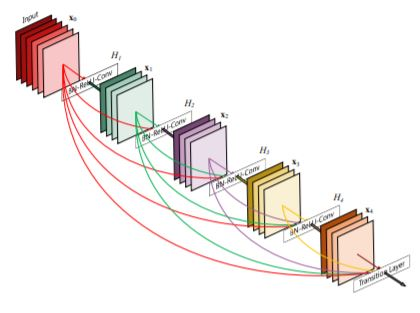
\includegraphics[width=.5\textwidth]{imagem/0x_densenet_block.jpg}
	% Caption centralizada
	\captionsetup{justification=centering}
	\captionfont{\small{\textbf{\\Fonte: \citeonline{liu-2017}.}}}	
	\label{fig:blocodenso}
\end{figure} 

Sendo assim, se cada camada do bloco possui uma saída de $x$ matrizes, o bloco possui $n$ camadas e a entrada do bloco possui tamanho $a$, a saída possuirá o tamanho representado pela Equação~\ref{eq:eq8}:

\begin{equation}
	\label{eq:eq8}	y = n x + a
\end{equation}

Vale mencionar que o valor de $x$ se conserva para toda a rede. Uma vantagem de usar blocos densos é a possibilidade de propagar informações com diversos níveis de abstração ao longo de toda a rede.

As \ac{DenseNet}s seguem um padrão arquitetural muito similar ao das \ac{ResNet}s começando a rede com uma camada de convolução $7\times7$ com \textit{strides} de $2\times2$ que é sucedida por uma camada de \textit{batch normalization} e outra de \ac{ReLU}. Depois disso, têm uma camada de \textit{pooling} pelo máximo e após essa camada, têm quatro blocos densos intercalados por blocos intermediários. Os blocos de convolução dentro dos blocos densos são compostos por uma camada de convolução $1\times1$ (que \citeonline{liu-2017} definem como camada de ``gargalo'') e uma camada de convolução $3\times3$. Vale mencionar que todas as camadas de convolução nos blocos densos são precedidas por uma camada de \textit{batch normalization} e \ac{ReLU}. Os blocos intermediários são compostos por uma camada de convolução $1\times1$ seguida de uma camada de \textit{pooling} pela média (que também é precedida por \textit{batch normalization} e \ac{ReLU}). No final dos 4 blocos densos, a rede possui mais uma camada de \textit{batch normalization} e \ac{ReLU} seguida por um \textit{pooling} pela média global e uma camada completamente conectada que faz a classificação. A Figura \ref{fig:archdensenet} mostra como é a arquitetura da rede.

\begin{figure}[H]
	% Alterar espaçamentos antes e depois do caption
	\setlength{\abovecaptionskip}{0pt}
	\setlength{\belowcaptionskip}{0pt}
	% Caption
	\caption[Arquitetura DenseNet]{Arquitetura DenseNet}
	\centering
	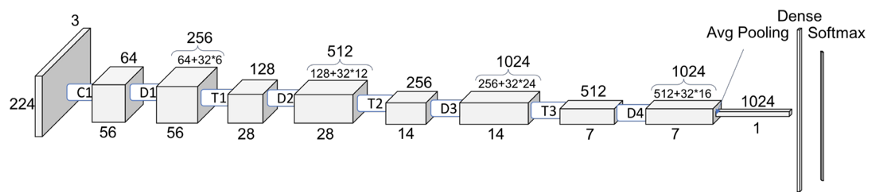
\includegraphics[width=.7\textwidth]{imagem/0x_densenet_arch.png}
	% Caption centralizada
	\captionsetup{justification=centering}
	\captionfont{\small{\textbf{\\Fonte: \citeonline{liu-2017}.}}}	
	\label{fig:archdensenet}
\end{figure}

O modelo proposto obteve resultados competitivos com os da literatura, ficando em segundo lugar no \ac{ILSVRC} de 2017 e apresentando resultados competitivos com os da literatura na época. O artigo também foi premiado como a melhor publicação da \ac{CVPR} do ano de 2017. O modelo obteve uma acurácia de 96\% na Cifar-10 e 82\% na Cifar-100.

\section{SSD: \textit{Single-Shot Multibox Detector}}
\label{secao:3:2}

\citeonline{wei-2015} propuseram um método a base de redes neurais convolucionais para fazer a localização e detecção de objetos. A proposta deles melhorou significativamente os resultados apresentados no estado da arte. Isso se deve ao fato de que eles não só conseguiram propor um modelo que faz a localização e classificação de forma eficiente (chegando a 74,3\% de \ac{mAP}), como conseguiram obter esse resultado fazendo classificação e localização em tempo real, com uma velocidade de 59 \ac{FPS}. Uma outra vantagem obtida por esse método é que ele consegue fazer a localização e classificação em imagens significativamente menores, uma vez que os quadros processados pelo \ac{YOLO} têm dimensões $448 \times 448$ e os processados pelo \ac{R-CNN} têm $1000\times 600$, o \ac{SSD} processa quadros de dimensões $300 \times 300$. Isso é uma vantagem, pois mesmo o algoritmo trabalhando com imagens menores, o resultado consegue competir com os outros métodos.

A abordagem consiste em utilizar a rede VGG16 \cite{simonyan-2014} como arquitetura base, substituir as camadas completamente conectadas fc6 e fc7 por camadas convolucionais, alterar o filtro pool5 de $2 \times 2 - s2$ para $3 \times 3 - s1$, e usaram o algoritmo \textit{à trous}\cite{holschneider-1990} para preencher os espaços vazios. Além disso, eles removeram todas as camadas de \textit{dropout} e a última camada completamente conectada. Por fim, as camadas de convolução geram os resultados de mais de 8000 localizações e classificações, as quais são filtradas em um passo final de supressão de não-máximos, que elimina todos os resultados com confiança abaixo de $0,5$.

A Figura \ref{fig:yoloxssd} mostra as diferenças entre as arquiteturas \ac{YOLO} e \ac{SSD}. Enquanto \citeonline{redmon-2015} usaram uma camada completamente conectada intermediária para fazer a localização dos objetos, \citeonline{wei-2015} usaram camadas de convolução sobre mapas de múltiplos tamanhos. Além disso, o \ac{SSD} trabalha com \textit{bounding-boxes} de tamanhos padrões $\{1, 2, 3, \frac{1}{2}, \frac{1}{3}\}$. Os filtros de convolução adicionais, os tamanhos padrões de \textit{bounding-boxes} e o uso de \textit{data-augmentation} foram cruciais na obtenção dos bons resultados.

  \begin{figure}[H]
	% Alterar espaçamentos antes e depois do caption
	\setlength{\abovecaptionskip}{0pt}
	\setlength{\belowcaptionskip}{0pt}
	% Caption
	\caption[YOLO e SSD]{Comparação entre \ac{YOLO} e \ac{SSD}}
	\centering
	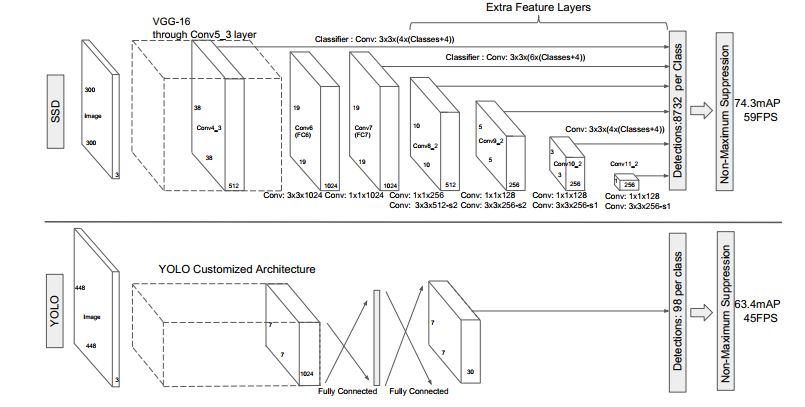
\includegraphics[width=.6\textwidth]{imagem/0x_yoloxssd.JPG}
	% Caption centralizada
	\captionsetup{justification=centering}
	\captionfont{\small{\textbf{\\Fonte: \citeonline{wei-2015}.}}}	
	\label{fig:yoloxssd}
\end{figure}

\section{DSSD: \textit{Deconvolution Single-Shot Detector}}
\label{secao:3:3}

\citeonline{cheng-2017} propuseram uma extensão do \ac{SSD}. Depois dos resultados obtidos pelo \ac{SSD} ao fazer localização e classificação de objetos com uma \ac{mAP} de $79,5\%$, eles propuseram uma abordagem alternativa, usando camadas de deconvolução ao final da rede. As camadas de deconvolução tem entre seus resultados o aumento de resolução do mapa de entrada. A abordagem visou explorar esse efeito com o intuito de aumentar a \ac{mAP} da classificação e localização de objetos, e, com isso, atingir uma \ac{mAP} de $81,5\%$. Embora essa abordagem tenha uma \ac{mAP} maior do que a obtida por \citeonline{wei-2015}, ela não é rápida o bastante pra fazer localização e classificação em tempo real.

A Figura \ref{fig:ssdxdssd} mostra as arquiteturas da \ac{SSD} e \ac{DSSD} mostrando as suas diferenças. É possível visualizar que a rede \ac{DSSD} utiliza as saídas da \ac{SSD} como entrada aos módulos de deconvolução.


\begin{figure}[H]
	% Alterar espaçamentos antes e depois do caption
	\setlength{\abovecaptionskip}{0pt}
	\setlength{\belowcaptionskip}{0pt}
	% Caption
	\caption[SSD e DSSD]{Comparação entre \ac{SSD} e \ac{DSSD}}
	\centering
	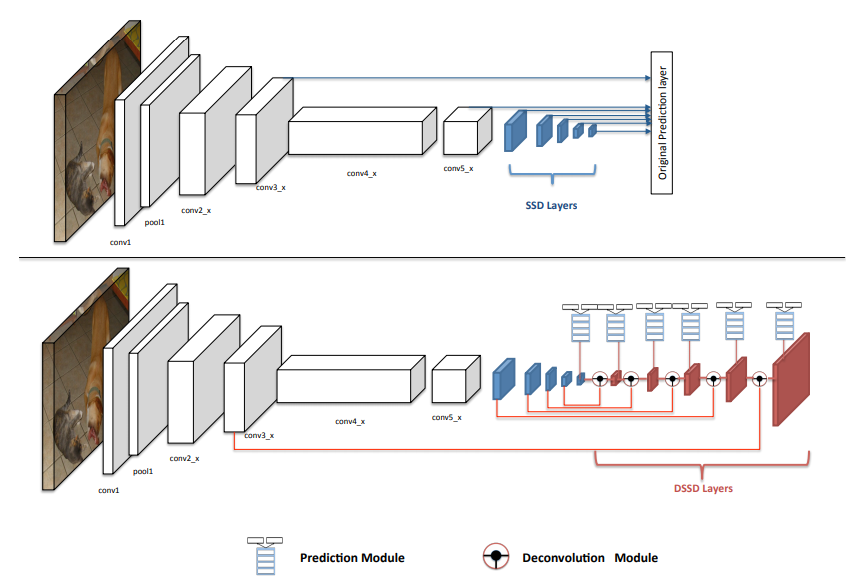
\includegraphics[width=.8\textwidth]{imagem/0x_comparacao_ssd_dssd.png}
	% Caption centralizada
	\captionsetup{justification=centering}
	\captionfont{\small{\textbf{\\Fonte: \citeonline{cheng-2017}.}}}	
	\label{fig:ssdxdssd}
\end{figure}

%Rever essa parte
Nesse trabalho, foram propostas duas alterações principais no modelo \ac{SSD}. A primeira delas foi a utilização da rede neural ResNet-101 \cite{he-2016}. \citeonline{cheng-2017} perceberam, porém, que apenas substituir a VGG16 pela \ac{ResNet} não produziria resultados melhores. Sendo assim, após adicionar as camadas de convolução do \ac{SSD} para fazer a detecção em múltiplos níveis, ele adicionou um módulo com mais algumas camadas de convolução a fim de melhorar os resultados. Os módulos propostos estão na Figura \ref{fig:ssdpred}.

\begin{figure}[H]
	% Alterar espaçamentos antes e depois do caption
	\setlength{\abovecaptionskip}{0pt}
	\setlength{\belowcaptionskip}{0pt}
	% Caption
	\caption[Módulos de predição SSD com ResNet]{Módulos de predição \ac{SSD} com \ac{ResNet}}
	\centering
	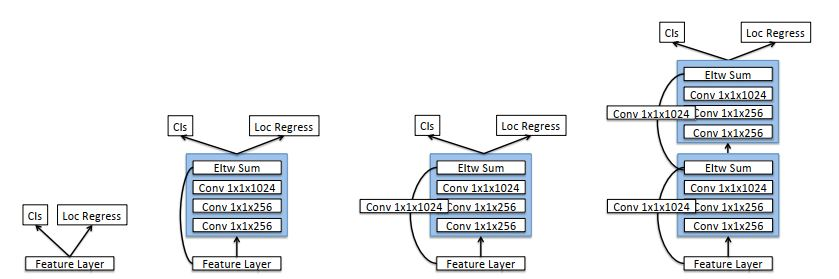
\includegraphics[width=.8\textwidth]{imagem/0x_dssdpredmod.jpg}
	% Caption centralizada
	\captionsetup{justification=centering}
	\captionfont{\small{\textbf{\\Fonte: \citeonline{cheng-2017}.}}}	
	\label{fig:ssdpred}
\end{figure}

Fazendo os testes, \citeonline{cheng-2017} perceberam que os melhores resultados foram obtidos usando a terceira opção que consistem um módulo residual com uma convolução na conexão alternativa e a junção das duas entradas sendo feita por meio de uma multiplicação elemento por elemento. Neste ponto, as mudanças ainda se mostravam pouco efetivas, já que a nova \ac{SSD}321 apresentava 77,1\% de \ac{mAP} contra 77,5\% de \ac{mAP} da \ac{SSD}300, ao passo que a nova \ac{SSD}513 apresentava 80,6\% contra 79,5\% da \ac{SSD}512.

Tendo isso em vista, após a implementação dos módulos \ac{SSD} na \ac{ResNet}101, \citeonline{cheng-2017} decidiram adicionar módulos usando camadas de deconvolução com o intuito de fazer um \textit{upsample} nas saídas da \ac{SSD} para obter mais dados. Depois de adicionar esses módulos, eles são combinados com o módulo \ac{SSD} anterior para gerar a nova saída. A Figura \ref{fig:deconv} mostra como é feita essa combinação.

\begin{figure}[H]
	% Alterar espaçamentos antes e depois do caption
	\setlength{\abovecaptionskip}{0pt}
	\setlength{\belowcaptionskip}{0pt}
	% Caption
	\caption[Módulos de deconvolução]{Módulos de deconvolução}
	\centering
	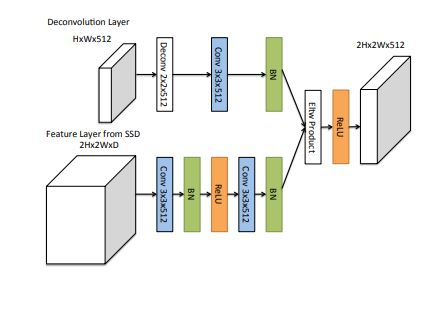
\includegraphics[width=.6\textwidth]{imagem/0x_dssd-deconv.jpg}
	% Caption centralizada
	\captionsetup{justification=centering}
	\captionfont{\small{\textbf{\\Fonte: \citeonline{cheng-2017}.}}}	
	\label{fig:deconv}
\end{figure}

Como mencionado anteriormente, embora o \ac{DSSD} tenha melhorado a \ac{mAP} do \ac{SSD}, ele não é aplicável para fazer a localização e classificação em tempo real. Com uma \ac{mAP} de $81,5\%$ ele consegue processar apenas $6,6$ \ac{FPS}. Isso se deve ao uso das deconvoluções, da ResNet 101 - que possui mais camadas, e, portanto toma mais tempo de processamento - e também ao aumento no número de \textit{bounding boxes} geradas($43688$ vs. $17080$), fazendo assim com que a supressão de não-máximos leve mais tempo.

\section{PASCAL VOC}
\label{secao:3:4}

Um grande desafio em treinar modelos de \textit{Deep Learning} é a necessidade de um grande volume de dados classificados manualmente. Com essa necessidade, diversos trabalhos foram desenvolvidos com o objetivo de apresentar uma base de dados anotados manualmente para um conjunto de problemas específicos. Nos trabalhos de Localização e classificação, uma das bases mais utilizadas é a \ac{PASCAL VOC}.

O desafio \ac{PASCAL VOC} foi realizado anualmente entre 2004 e 2012, e a cada ano novas imagens e novos desafios foram propostos na área de visão computacional. Os principais desafios envolviam Localização e Classificação de Objetos, Segmentação Semântica, \textit{layout} humano (um desafio que consiste em detectar partes do corpo como cabeça, mãos e pés) e classificação de ações \cite{everingham-2015}.

O desafio de Localização e Classificação de objetos desde 2007 possui 20 classes distintas de objetos e a cada ano eles criaram uma nova base com mais imagens extraídas da internet. A Tabela \ref{tab:voc2007} mostra as classes, o número de imagens e o número de objetos por classe nos conjuntos de treino, validação e teste.

\begin{table}[H]
	\centering
	\footnotesize
	% Alterar espaçamentos antes e depois do caption
	\setlength{\abovecaptionskip}{0pt}
	\setlength{\belowcaptionskip}{0pt}
	% Caption
	\caption[Pascal VOC 2007]{Classes de imagens do PASCAL VOC 2007}
	\label{tab:voc2007}
	\begin{tabular}{l|l|l|l|l|l|l|ll}
		& \multicolumn{2}{l|}{Treino} & \multicolumn{2}{l|}{Validação} & \multicolumn{2}{l|}{Treino/Validação} & \multicolumn{2}{l}{Teste}              \\ \hline
		& imagens      & Objetos      & Imagens        & Objetos       & Imagens           & Objetos           & \multicolumn{1}{l|}{Imagens} & Objetos \\ \hline
		Avião          & 112          & 151          & 126            & 155           & 238               & 306               & \multicolumn{1}{l|}{204}     & 285     \\
		Bicicleta      & 116          & 176          & 127            & 177           & 243               & 353               & \multicolumn{1}{l|}{239}     & 282     \\
		Pássaro        & 180          & 243          & 150            & 243           & 330               & 486               & \multicolumn{1}{l|}{282}     & 459     \\
		Barco          & 81           & 140          & 100            & 150           & 181               & 290               & \multicolumn{1}{l|}{172}     & 263     \\
		Garrafa        & 139          & 253          & 105            & 252           & 244               & 505               & \multicolumn{1}{l|}{212}     & 469     \\
		Ônibus         & 97           & 115          & 89             & 114           & 186               & 229               & \multicolumn{1}{l|}{174}     & 213     \\
		Carro          & 376          & 625          & 337            & 625           & 713               & 1250              & \multicolumn{1}{l|}{721}     & 1201    \\
		Gato           & 163          & 186          & 174            & 190           & 337               & 376               & \multicolumn{1}{l|}{322}     & 358     \\
		Cadeira        & 224          & 400          & 221            & 398           & 445               & 798               & \multicolumn{1}{l|}{417}     & 756     \\
		Vaca           & 69           & 136          & 72             & 123           & 141               & 259               & \multicolumn{1}{l|}{127}     & 244     \\
		Mesa de Jantar & 97           & 103          & 103            & 112           & 200               & 215               & \multicolumn{1}{l|}{190}     & 206     \\
		Cão            & 203          & 253          & 218            & 257           & 421               & 510               & \multicolumn{1}{l|}{418}     & 489     \\
		Cavalo         & 139          & 182          & 148            & 180           & 287               & 362               & \multicolumn{1}{l|}{274}     & 348     \\
		Motocicleta    & 120          & 167          & 125            & 172           & 245               & 339               & \multicolumn{1}{l|}{222}     & 325     \\
		Pessoa         & 1025         & 2358         & 983            & 2332          & 2008              & 4690              & \multicolumn{1}{l|}{2007}    & 4528    \\
		Vaso de planta & 133          & 248          & 112            & 266           & 245               & 514               & \multicolumn{1}{l|}{224}     & 480     \\
		Ovelha         & 48           & 130          & 48             & 127           & 96                & 257               & \multicolumn{1}{l|}{97}      & 242     \\
		Sofá           & 111          & 124          & 118            & 124           & 229               & 248               & \multicolumn{1}{l|}{223}     & 239     \\
		Trem           & 127          & 145          & 134            & 152           & 261               & 297               & \multicolumn{1}{l|}{259}     & 282     \\
		Monitor/TV     & 128          & 166          & 128            & 158           & 256               & 324               & \multicolumn{1}{l|}{299}     & 308     \\
		Total          & 2501         & 6301         & 2510           & 6307          & 5011              & 12608             & \multicolumn{1}{l|}{4952}    & 12032  
	\end{tabular}
	\\
	\captionfont{\small{\textbf{\\Fonte: Adaptado de \citeonline{everingham-2010}.}}}
\end{table}

Analisando a tabela é possível perceber que a base é desbalanceada. A classe pessoa, por exemplo, está presente em mais de 1000 imagens e tem mais de 2000 instâncias apenas no conjunto de treinamento. Enquanto isso, a classe ovelha aparece apenas 130 vezes em 48 imagens no conjunto de treinamento. Esse desbalanceamento pode ser um desafio durante o treinamento caso o modelo não seja robusto. A Figura \ref{fig:pascal2007} mostra exemplos das classes presentes na \ac{PASCAL VOC} 2007.

\begin{figure}[H]
	% Alterar espaçamentos antes e depois do caption
	\setlength{\abovecaptionskip}{0pt}
	\setlength{\belowcaptionskip}{0pt}
	% Caption
	\caption[Imagens PASCAL VOC 2007]{Exemplos de imagens da PASCAL VOC 2007}
	\centering
	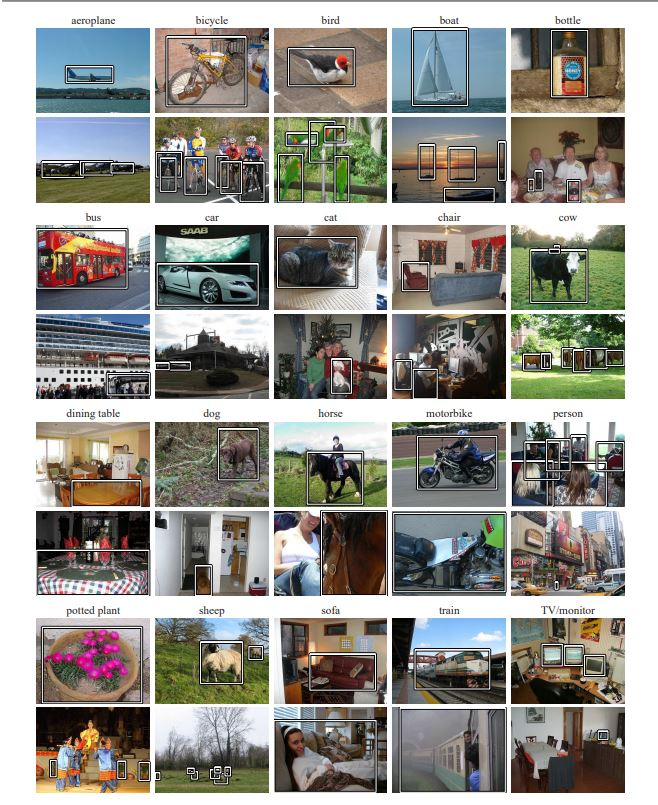
\includegraphics[width=.9\textwidth]{imagem/0x_pascal2007.jpg}
	% Caption centralizada
	\captionsetup{justification=centering}
	\captionfont{\small{\textbf{\\Fonte: \citeonline{everingham-2010}.}}}	
	\label{fig:pascal2007}
\end{figure}

\subsection{PASCAL VOC 2012}
\label{section:3:4:1}

Em 2012 foi lançado uma outra versão da \ac{PASCAL VOC}. Essa edição da competição tinha uma base de dados maior e mais robusta, embora ainda mantivesse as mesmas 20 classes da base de 2007. A Tabela \ref{tab:voc2012} mostra a distribuição de imagens e objetos na base \ac{PASCAL VOC} 2012. Nela será possível perceber o mesmo desbalanceamento encontrado na base de 2007. Porém, uma vantagem é que ela tem mais imagens, se comparada à base de 2007. Além disso, como as bases são completamente distintas, podem ser usadas em conjunto para o treinamento e a validação dos modelos.

\begin{table}[H]
	\centering
	\footnotesize
	% Alterar espaçamentos antes e depois do caption
	\setlength{\abovecaptionskip}{0pt}
	\setlength{\belowcaptionskip}{0pt}
	% Caption
	\caption[Pascal VOC 2012]{Classes de imagens do PASCAL VOC 2012}
	\label{tab:voc2012}
	\begin{tabular}{l|l|l|l|l|l|l}
		& \multicolumn{2}{l|}{Treino} & \multicolumn{2}{l|}{Validação} & \multicolumn{2}{l}{Treino/Validação} \\ \hline
		& imagens      & Objetos      & Imagens        & Objetos       & Imagens           & Objetos           \\ \hline
		Avião          & 327          & 432          & 343            & 433           & 670               & 865               \\
		Bicicleta      & 268          & 353          & 284            & 358           & 552               & 711               \\
		Pássaro        & 395          & 560          & 370            & 559           & 765               & 1119              \\
		Barco          & 260          & 426          & 248            & 424           & 508               & 850               \\
		Garrafa        & 365          & 629          & 341            & 630           & 706               & 1259              \\
		Ônibus         & 213          & 292          & 208            & 301           & 421               & 593               \\
		Carro          & 590          & 1013         & 571            & 1004          & 1161              & 2017              \\
		Gato           & 539          & 605          & 541            & 612           & 1080              & 1217              \\
		Cadeira        & 566          & 1178         & 553            & 1176          & 1119              & 2354              \\
		Vaca           & 151          & 290          & 152            & 298           & 303               & 588               \\
		Mesa de Jantar & 269          & 304          & 269            & 305           & 538               & 609               \\
		Cão            & 632          & 756          & 654            & 759           & 1286              & 1515              \\
		Cavalo         & 237          & 350          & 245            & 360           & 482               & 710               \\
		Motocicleta    & 265          & 357          & 261            & 356           & 526               & 713               \\
		Pessoa         & 1994         & 4194         & 2093           & 4372          & 4087              & 8566              \\
		Vaso de planta & 269          & 484          & 258            & 489           & 527               & 973               \\
		Ovelha         & 171          & 400          & 154            & 413           & 325               & 813               \\
		Sofá           & 257          & 281          & 250            & 285           & 507               & 566               \\
		Trem           & 273          & 313          & 271            & 315           & 544               & 628               \\
		Monitor/TV     & 290          & 392          & 285            & 392           & 575               & 784               \\
		Total          & 5717         & 13609        & 5823           & 13841         & 11540             & 27450            
	\end{tabular}
\\
\captionfont{\small{\textbf{\\Fonte: Adaptado de \citeonline{everingham-2011}.}}}
\end{table}

\subsection{Métricas}
\label{section:3:4:2}

A principal métrica utilizada para avaliar trabalhos de Localização e Classificação é a \ac{mAP}. Para deduzir o \ac{mAP}, é necessário definir os conceitos de Precisão e Revocação. Então seja $TP$ os verdadeiros positivos encontrados por um modelo, $FN$ os falsos negativos e $FP$ os falsos positivos (os verdadeiros negativos não entram no cálculo pois os modelos não são treinados com base no \textit{ground-truth} do \textit{background}). A Precisão $P$ pode ser definida pela Equação \ref{eq:eq9}.

\begin{equation}
	\label{eq:eq9}
	P = \dfrac{TP}{TP+FP}
\end{equation}

\noindent
Ao passo que a revocação $R$ pode ser definida pela Equação \ref{eq:eq10}.

\begin{equation}
	\label{eq:eq10}
	R = \dfrac{TP}{TP+FN}
\end{equation}

Uma vez que se tenha os valores de precisão e revocação, é traçada a curva $P \times R$. Essa curva se comporta com $R$ aumentando a medida que aumentam os falsos negativos e com $P$ oscilando e fazendo ``zigue-zague''. O valor teórico da Precisão média é determinado pela área sobre a curva $P \times R$ como está descrito na Equação \ref{eq:eq11}.

\begin{equation}
	\label{eq:eq11}
	AP = \int_{0}^{1}P(R)dR
\end{equation}

Porém, como mencionado anteriormente, a curva $P \times R$ se comporta de forma não-linear fazendo ``zigue-zague''. Esse comportamento dificulta um cálculo preciso da área sobre a curva. Para contornar essa dificuldade, \citeonline{salton-1986} propuseram que o valor da precisão média fosse interpolado de acordo com a Equação \ref{eq:eq12}

\begin{equation}
	\label{eq:eq12}
	AP = \dfrac{1}{11} \sum_{R_i \in \{0.0, 0.1, .. 1.0\}} max(P(R_i))
\end{equation}

\citeonline{everingham-2015} porém começaram a adotar uma forma diferente de calcular a integral a partir de 2010. Ao invés de fazer a interpolação como na Equação \ref{eq:eq12}, eles passaram a calcular a integral pela regra dos trapézios, definida pela Equação \ref{eq:eq13}.

\begin{equation}
	\label{eq:eq13}
	AP = \dfrac{0.1}{2}[P(R_0) + P(R_1) + 2.\sum_{R_i \in \{0.1, 0.2, .., 0.9\}}P(R_i)]
\end{equation}

Sendo assim, o \ac{mAP} pode ser definido como a média das precisões médias por classe.